\documentclass[11pt]{article} 
\usepackage[english]{babel}
\usepackage[utf8]{inputenc}
\usepackage[margin=0.5in]{geometry}
\usepackage{amsmath}
\usepackage{amsthm}
\usepackage{amsfonts}
\usepackage{amssymb}
\usepackage[usenames,dvipsnames]{xcolor}
\usepackage{graphicx}
\usepackage[siunitx]{circuitikz}
\usepackage{tikz}
\usepackage{tkz-berge}
\usetikzlibrary{positioning, automata, backgrounds}
\usepackage[colorinlistoftodos, color=orange!50]{todonotes}
\usepackage{hyperref}
\usepackage[numbers, square]{natbib}
\usepackage{fancybox}
\usepackage{epsfig}
\usepackage{soul}
\usepackage[framemethod=tikz]{mdframed}
\usepackage[shortlabels]{enumitem}
\usepackage[version=4]{mhchem}
\usepackage{multicol}
\usepackage{forest}
\usepackage{mathtools}
\DeclareUnicodeCharacter{2212}{\textendash}
\usepackage{comment}
\usepackage{enumitem}
\usepackage[utf8]{inputenc}
\usepackage{listings}
\usepackage{color}
\usepackage[numbers]{natbib}
\usepackage{subfiles}
\usepackage{tkz-berge}
\usepackage{algorithm}
\usepackage[noend]{algpseudocode}


\newtheorem{prop}{Proposition}[section]
\newtheorem{thm}{Theorem}[section]
\newtheorem{lemma}{Lemma}[section]
\newtheorem{cor}{Corollary}[prop]

\theoremstyle{definition}
\newtheorem{definition}{Definition}

\theoremstyle{definition}
\newtheorem{required}{Problem}

\theoremstyle{definition}
\newtheorem{ex}{Example}

\newcommand{\interval}[4]{\draw (#2, #1) -- (#3, #1); % Usage: \interval{height}{start}{end}{label}
\draw (#2, #1-0.11) -- (#2, #1+0.11); % draw left whisker
\draw (#3, #1-0.11) -- (#3, #1+0.11); % draw right whisker
\node[] at (#2-0.25, #1) {#4};
}


\setlength{\marginparwidth}{3.4cm}
%#########################################################

%To use symbols for footnotes
\renewcommand*{\thefootnote}{\fnsymbol{footnote}}
%To change footnotes back to numbers uncomment the following line
%\renewcommand*{\thefootnote}{\arabic{footnote}}

% Enable this command to adjust line spacing for inline math equations.
% \everymath{\displaystyle}

% _______ _____ _______ _      ______ 
%|__   __|_   _|__   __| |    |  ____|
%   | |    | |    | |  | |    | |__   
%   | |    | |    | |  | |    |  __|  
%   | |   _| |_   | |  | |____| |____ 
%   |_|  |_____|  |_|  |______|______|
%%%%%%%%%%%%%%%%%%%%%%%%%%%%%%%%%%%%%%%

\title{
\normalfont \normalsize 
\textsc{CSCI 3104 Fall 2021 \\ 
Instructors: Profs. Grochow and Waggoner} \\
[10pt] 
\rule{\linewidth}{0.5pt} \\[6pt] 
\huge Problem Set 9 \\
\rule{\linewidth}{2pt}  \\[10pt]
}
%\author{Your Name}
\date{}

\begin{document}
\definecolor {processblue}{cmyk}{0.96,0,0,0}
\maketitle


%%%%%%%%%%%%%%%%%%%%%%%%%
%%%%%%%%%%%%%%%%%%%%%%%%%%
%%%%%%%%%%FILL IN YOUR NAME%%%%%%%
%%%%%%%%%%AND STUDENT ID%%%%%%%%
%%%%%%%%%%%%%%%%%%%%%%%%%%
\noindent
Due Date \dotfill TODO \\
Name \dotfill \textbf{John Blackburn} \\
Student ID \dotfill \textbf{jobl2177} \\
Collaborators \dotfill \textbf{List Your Collaborators Here}

\tableofcontents

\section{Instructions}
 \begin{itemize}
	\item The solutions \textbf{must be typed}, using proper mathematical notation. We cannot accept hand-written solutions. \href{http://ece.uprm.edu/~caceros/latex/introduction.pdf}{Here's a short intro to \LaTeX.}
	\item You should submit your work through the \textbf{class Canvas page} only. Please submit one PDF file, compiled using this \LaTeX \ template.
	\item You may not need a full page for your solutions; pagebreaks are there to help Gradescope automatically find where each problem is. Even if you do not attempt every problem, please submit this document with no fewer pages than the blank template (or Gradescope has issues with it).

	\item You are welcome and encouraged to collaborate with your classmates, as well as consult outside resources. You must \textbf{cite your sources in this document.} \textbf{Copying from any source is an Honor Code violation. Furthermore, all submissions must be in your own words and reflect your understanding of the material.} If there is any confusion about this policy, it is your responsibility to clarify before the due date. 

	\item Posting to \textbf{any} service including, but not limited to Chegg, Reddit, StackExchange, etc., for help on an assignment is a violation of the Honor Code.

	\item You \textbf{must} virtually sign the Honor Code (see Section \ref{HonorCode}). Failure to do so will result in your assignment not being graded.
\end{itemize}


\section{Honor Code (Make Sure to Virtually Sign)} \label{HonorCode}

\begin{required}
\begin{itemize}
\item My submission is in my own words and reflects my understanding of the material.
\item Any collaborations and external sources have been clearly cited in this document.
\item I have not posted to external services including, but not limited to Chegg, Reddit, StackExchange, etc.
\item I have neither copied nor provided others solutions they can copy.
\end{itemize}

%\noindent In the specified region below, clearly indicate that you have upheld the Honor Code. Then type your name. 
\end{required}

\begin{proof}[Agreed john blackburn.]
%% Typing "I agree to the above," followed by your name is sufficient.
\end{proof}


\newpage
\section{Standard 24- Dynamic Programming: Design DP Algorithms}

\begin{required}
The \textsf{Highest Reflective Subsequence} problem is defined as follows.
\begin{itemize}
\item \textsf{Instance:} A string $\omega \in \Sigma^{n}$, where $\Sigma$ is our fixed alphabet.
\item \textsf{Solution:} A subsequence $\psi \in \Sigma^{\ell}$ of $\omega$ of maximum length such that for all $i \in \{1, \ldots, \ell\}$, $\psi_{i} = \psi_{\ell - i + 1}$.
\end{itemize}


\noindent \\ The goal of this problem set is to design a dynamic programming algorithm to solve the \textsf{Highly Reflective Subsequence} problem.

\begin{enumerate}[label=(\alph*)]
\subsection{Problem 2\ref{2a}}
\item \label{2a} Let $L[i, j]$ denote the length of the highest reflective subsequence of $\omega[i, \ldots, j]$. Write down a mathematical recurrence for $L[i, j]$. Clearly justify each case.

\begin{proof}[Answer]
%Your answer here



$$
L[i,j] =\begin{cases}
 0 & \text{if $i>j $} \\  
 1 & \text{if $i=j$} \\  
 L[i+1,j-1] + 2 & \text{if $i,j>0$,  $\omega[i] = \omega[j] $}  \\
 MAX(L[i+1,j], L[i,j-1]) & \text{if $i,j>0$, $\omega[i]  != \omega[j]$}
		 \end{cases}
$$

The base cases occur when $i =j $ and when $i>j$. if $i = j$ we know the length of the subsequence must be 1 since $i$ and $j$ are in the same spot of $\omega$. As for when $i>j$ we know that the subsequence will be of length 0 because the sequence cannot be a palindrome when $i>j$. 

Now for the recursive cases: They can be broken into two cases, them being when the outer two letters are equivalent and when they are not. When $\omega[i] = \omega[j] $ we know that the subsequence will be 2 links longer than the subsequence of the string $\omega$ where $i = i +1$ and $j = j -1$. This effectively is saying we take the subsequence from the string $\omega$ without the outer two letters and add 2 to its length because the last and first letters of the new string are equivalent. As for when $\omega[i]  != \omega[j]$ we take the max of the two subsequences that make up the inside of the current string we have, one string including $i$ up to $j-1$, and the other including $j$ going down to $i+1$.

\end{proof}



\newpage
\subsection{Problem 2\ref{2b}}
\item \label{2b} Clearly describe how to construct and fill in the lookup table. For the cell $L[i, j]$, clearly describe the sub-cases we consider, which optimal sub-case we select, and any relevant pointers that should be included in the table.

\begin{proof}[Answer]
%Your answer here\


 Let w be our input string of length n. We initialize a lookup table $T[0,...,n][0,...,n]$ to be a two-dimensional array, where each cell stores:
A natural number which indicates the max length of a palindrome sequence at that length

The first row and column are both filled with the letters of the input string. let the string along the row be denoted as w and the string along the column be denoted by t. 

let i denote the row number and j denote the column number.

We now proceed to fill in the cells in a bottom up manner, row-by-row, the cells $T[i][j]$ are filled as follows.

Case 1 : suppose the cell we are looking at is where $i=j$. For example $T[1][1]$ or $T[3][3]$. So, in this case we always set:
-Set $T [i][j]$.length $=  1$; 

Case 2: suppose $i>j$. For these cases we set:
- Set T [i][j].length = 0; 



Case 3: Suppose $w_i = t_j$ . This tells us that the characters at this subproblem are equivalent and should 
be added to our sequence. So we take the following actions:
-Set $T [i][j]$.length$ =$ $T [i + 1][j − 1]$.length $+ 2$;\







Case 4: Suppose $w_i != t_j$ . We need to consider the two subproblems, whose solutions are stored in: T [i+ 1][j] and T [i][j − 1], respectively. 


If T [i + 1][j].length $\geq $T [i][j − 1].length, we set:

– T[i][j].length=T[i+1][j].length


 Otherwise, we set:
– T[i][j].length=T[i][j−1].length 

\

The table gives us the max length of our highest reflective subsequence at T[0][n-1]. No pointers are neccessary with this lookup table to find the length of our subsequence. 
\end{proof}



\newpage
\subsection{Problem 2\ref{2c}}
\item \label{2c} Work through an example of your algorithm using the input string $\omega = \texttt{abcdeca}$. Clearly show how to recover an optimal solution using your lookup table. You may hand-draw your lookup table, but your explanation must be typed.

\begin{proof}[Answer]
%Your answer here
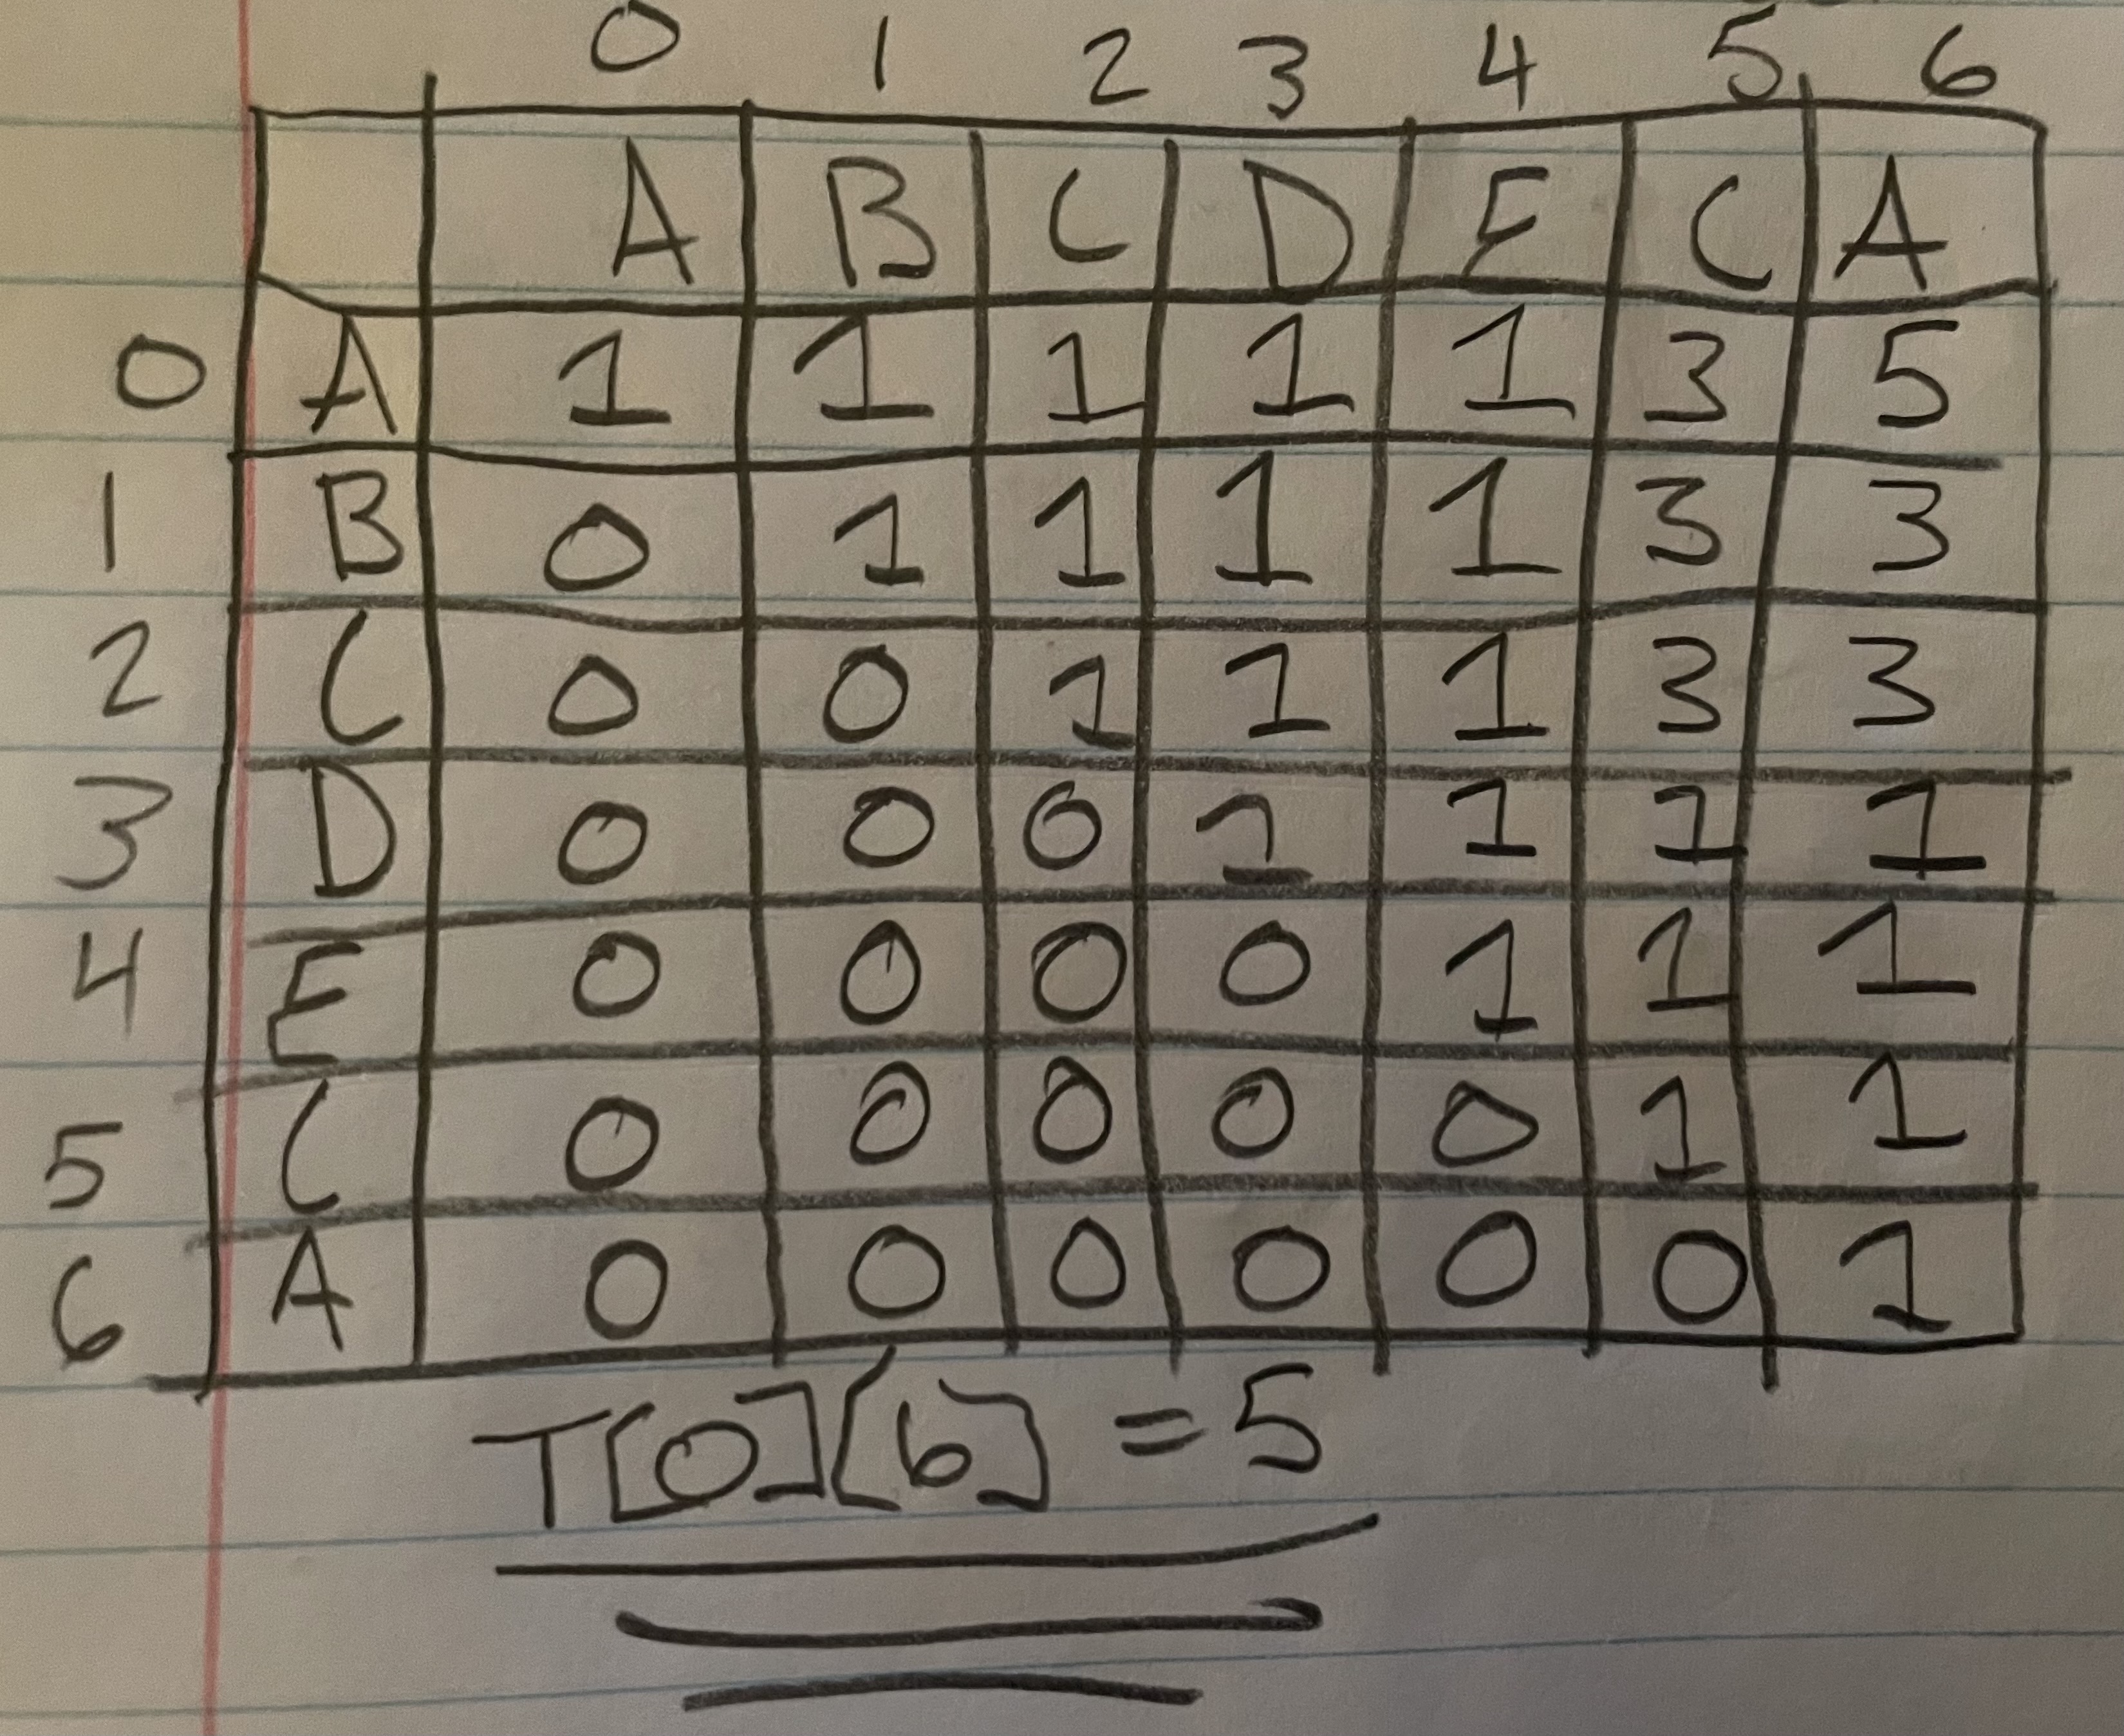
\includegraphics[width = 15cm]{IMG-4903.jpg}
I worked through the above input string and made a table for it. I started at the bottom left of the table and made my way across the row and then went up and across each row and finally finished at T[0][6] to get the final answer of 5. My answer means that the highest reflective subsequence of the input string has a length of 5. This table structure works becuase each new problem builds on the previous subproblems before it. Leaving the final problem having built upon all the previous ones giving the final answer in the final box. You can only solve the final problem in the table when every previous subproblem has been completed. 
\end{proof}

\end{enumerate}



\end{required}

\end{document} % NOTHING AFTER THIS LINE IS PART OF THE DOCUMENT



